\section{Испытания на уязвимых образцах}

Для проверки работы фаззера были проведены испытания на нескольких уязвимых образцах программ. Описание этих испытаний будут приведены далее. На фаззинг каждого перечисленного примера отводилось не более 30 минут.

\subsection{Уязвимые программы}

Первым исполняемым файлом, для которого проводилось тестирование, является парсер exif -- распространённого формата контейнера графических данных. Для исследования фаззер запускается в бинарном режиме, то есть для своей работы основывается на наборе начальных тестовых примеров. Применимо к парсеру exif, начальным тестовым примером является созданное в программе GIMP цветное изображение размером 4x4 пикселя, хранимое в формате jpeg. Исполняемый файл был скомпилирован из исходного кода на языке Си, каких-либо модификаций не вносилось.

Вторым исследуемым файлом стал парсер json. Для его формирования в корректно написанную программу были внесены несколько ошибок, связанных с неверной аллокацией памяти и граничными условиями циклов. Для генерации входных данных была использована следующая описывающая синтаксис json грамматика:

\begin{code}
root -> jsonobj;
jsonobj -> string 
    | number 
    | list 
    | dict 
    | null;
string -> "\"" re("[\x20-\x4f]*") "\"";
number -> re("[-]?[0-9]*[.]?[0-9]+");
list -> "[" listItems "]";
listItems -> jsonobj 
    | jsonobj moreListItems 
    | Nothing;
moreListItems -> "," jsonobj moreListItems 
    | Nothing;
dict -> "{" dictItems "}";
dictItems -> Nothing 
    | dictEntry 
    | dictEntry moreDictEntries;
moreDictEntries -> "," dictEntry moreDictEntries 
    | Nothing;
dictEntry -> string ":" jsonobj;
null -> "null";
\end{code}

\subsection{Результаты фаззинга}

Фаззинг парсера exif позволил выявить 179 уникальных путей и 21 уникальный краш. Система демонстрирует классическое для фаззеров поведение -- время между обнаружениями новых путей постепенно снижается и поиск выходит на плато (рисунок \ref{fig:fuzzing-speed}, точками отмечено обнаружение новых уникальных крашей).

\begin{figure}[h]
	\centering
	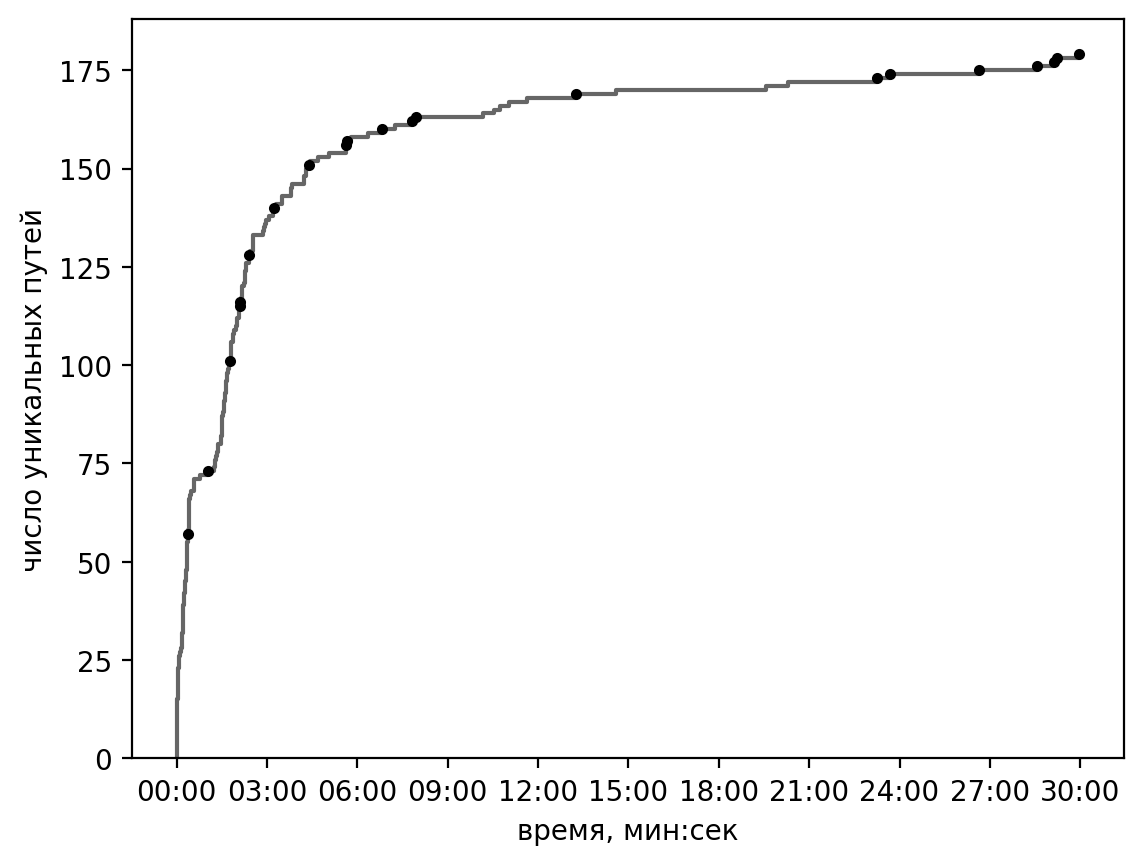
\includegraphics[width=0.8\textwidth]{fuzzing-speed.png}
	\caption{Обнаружение новых путей с течением времени}
	\label{fig:fuzzing-speed}
\end{figure}%

Фаззинг парсера json привёл к генерации тестовых примеров, затрагивающих каждую из внесённых в исполняемый файл ошибок. Стоит отметить, что фаззинг парсера json привёл к генерации большого числа уникальных с точки зрения системы ошибок, превышающего количество внесённых. Это вызвано простотой системы для идентификации уникальных крашей. Одним из вариантов решения данной проблемы является минимизация крашей также на уровне пути в программе: если удаётся обнаружить новый, как кажется, тестовый пример, стоит выполнить полную трассировку на нём и добавить в библиотеку, исключив из неё краши, которые происходят в том же месте и пути выполнения которых включают в себя обнаруженный.
